A very high-level overview of the topic is given here.

\lipsum[1]

\section{circRNAs}
This section describes what circRNAs are, how they are formed, and what their functions are.
It also gives insights into the current state of research.

\subsection{Biogenesis}
During standard gene expression, pre-mRNA is transcribed from DNA.
Splicing then removes introns and joins exons to produce mature mRNA \supercite{black_mechanisms_2003}.
In conventional splicing, an upstream 5' splice site (donor) connects to a downstream 3' splice site (acceptor), forming linear mRNA (\cref{fig:circRNA_splicing}a).
Conversely, for circRNAs, a downstream 5' splice site connects to an upstream 3' splice site in reverse order across at least one exon \supercite{chen_expanding_2020}.
This backsplicing process creates a circular RNA molecule (\cref{fig:circRNA_splicing}b).

\subsubsection{Circular intronic RNAs}
Introns excised during conventional splicing typically form a lariat shape, which is usually debranched and degraded shortly after splicing (\cref{fig:circRNA_splicing}a).
However, some introns avoid debranching and instead form covalent circular RNA molecules (\cref{fig:circRNA_splicing}c).
These are known as circular intronic RNAs (ciRNAs) \supercite{chen_expanding_2020,zhang_circular_2013}.

\subsubsection{Alternative splicing}
In conventional splicing, introns are removed and exons are joined linearly.
However, in some cases, exons are skipped or introns are retained, leading to alternative mature mRNA transcripts based on the same pre-mRNA.
This process is known as alternative splicing \supercite{nilsen_expansion_2010}.
Similarly, circRNAs can be subject to alternative splicing. This can result in the structures shown in \cref{fig:circRNA_splicing}e and \cref{fig:circRNA_splicing}f.

\begin{figure}[h]
    \centering
    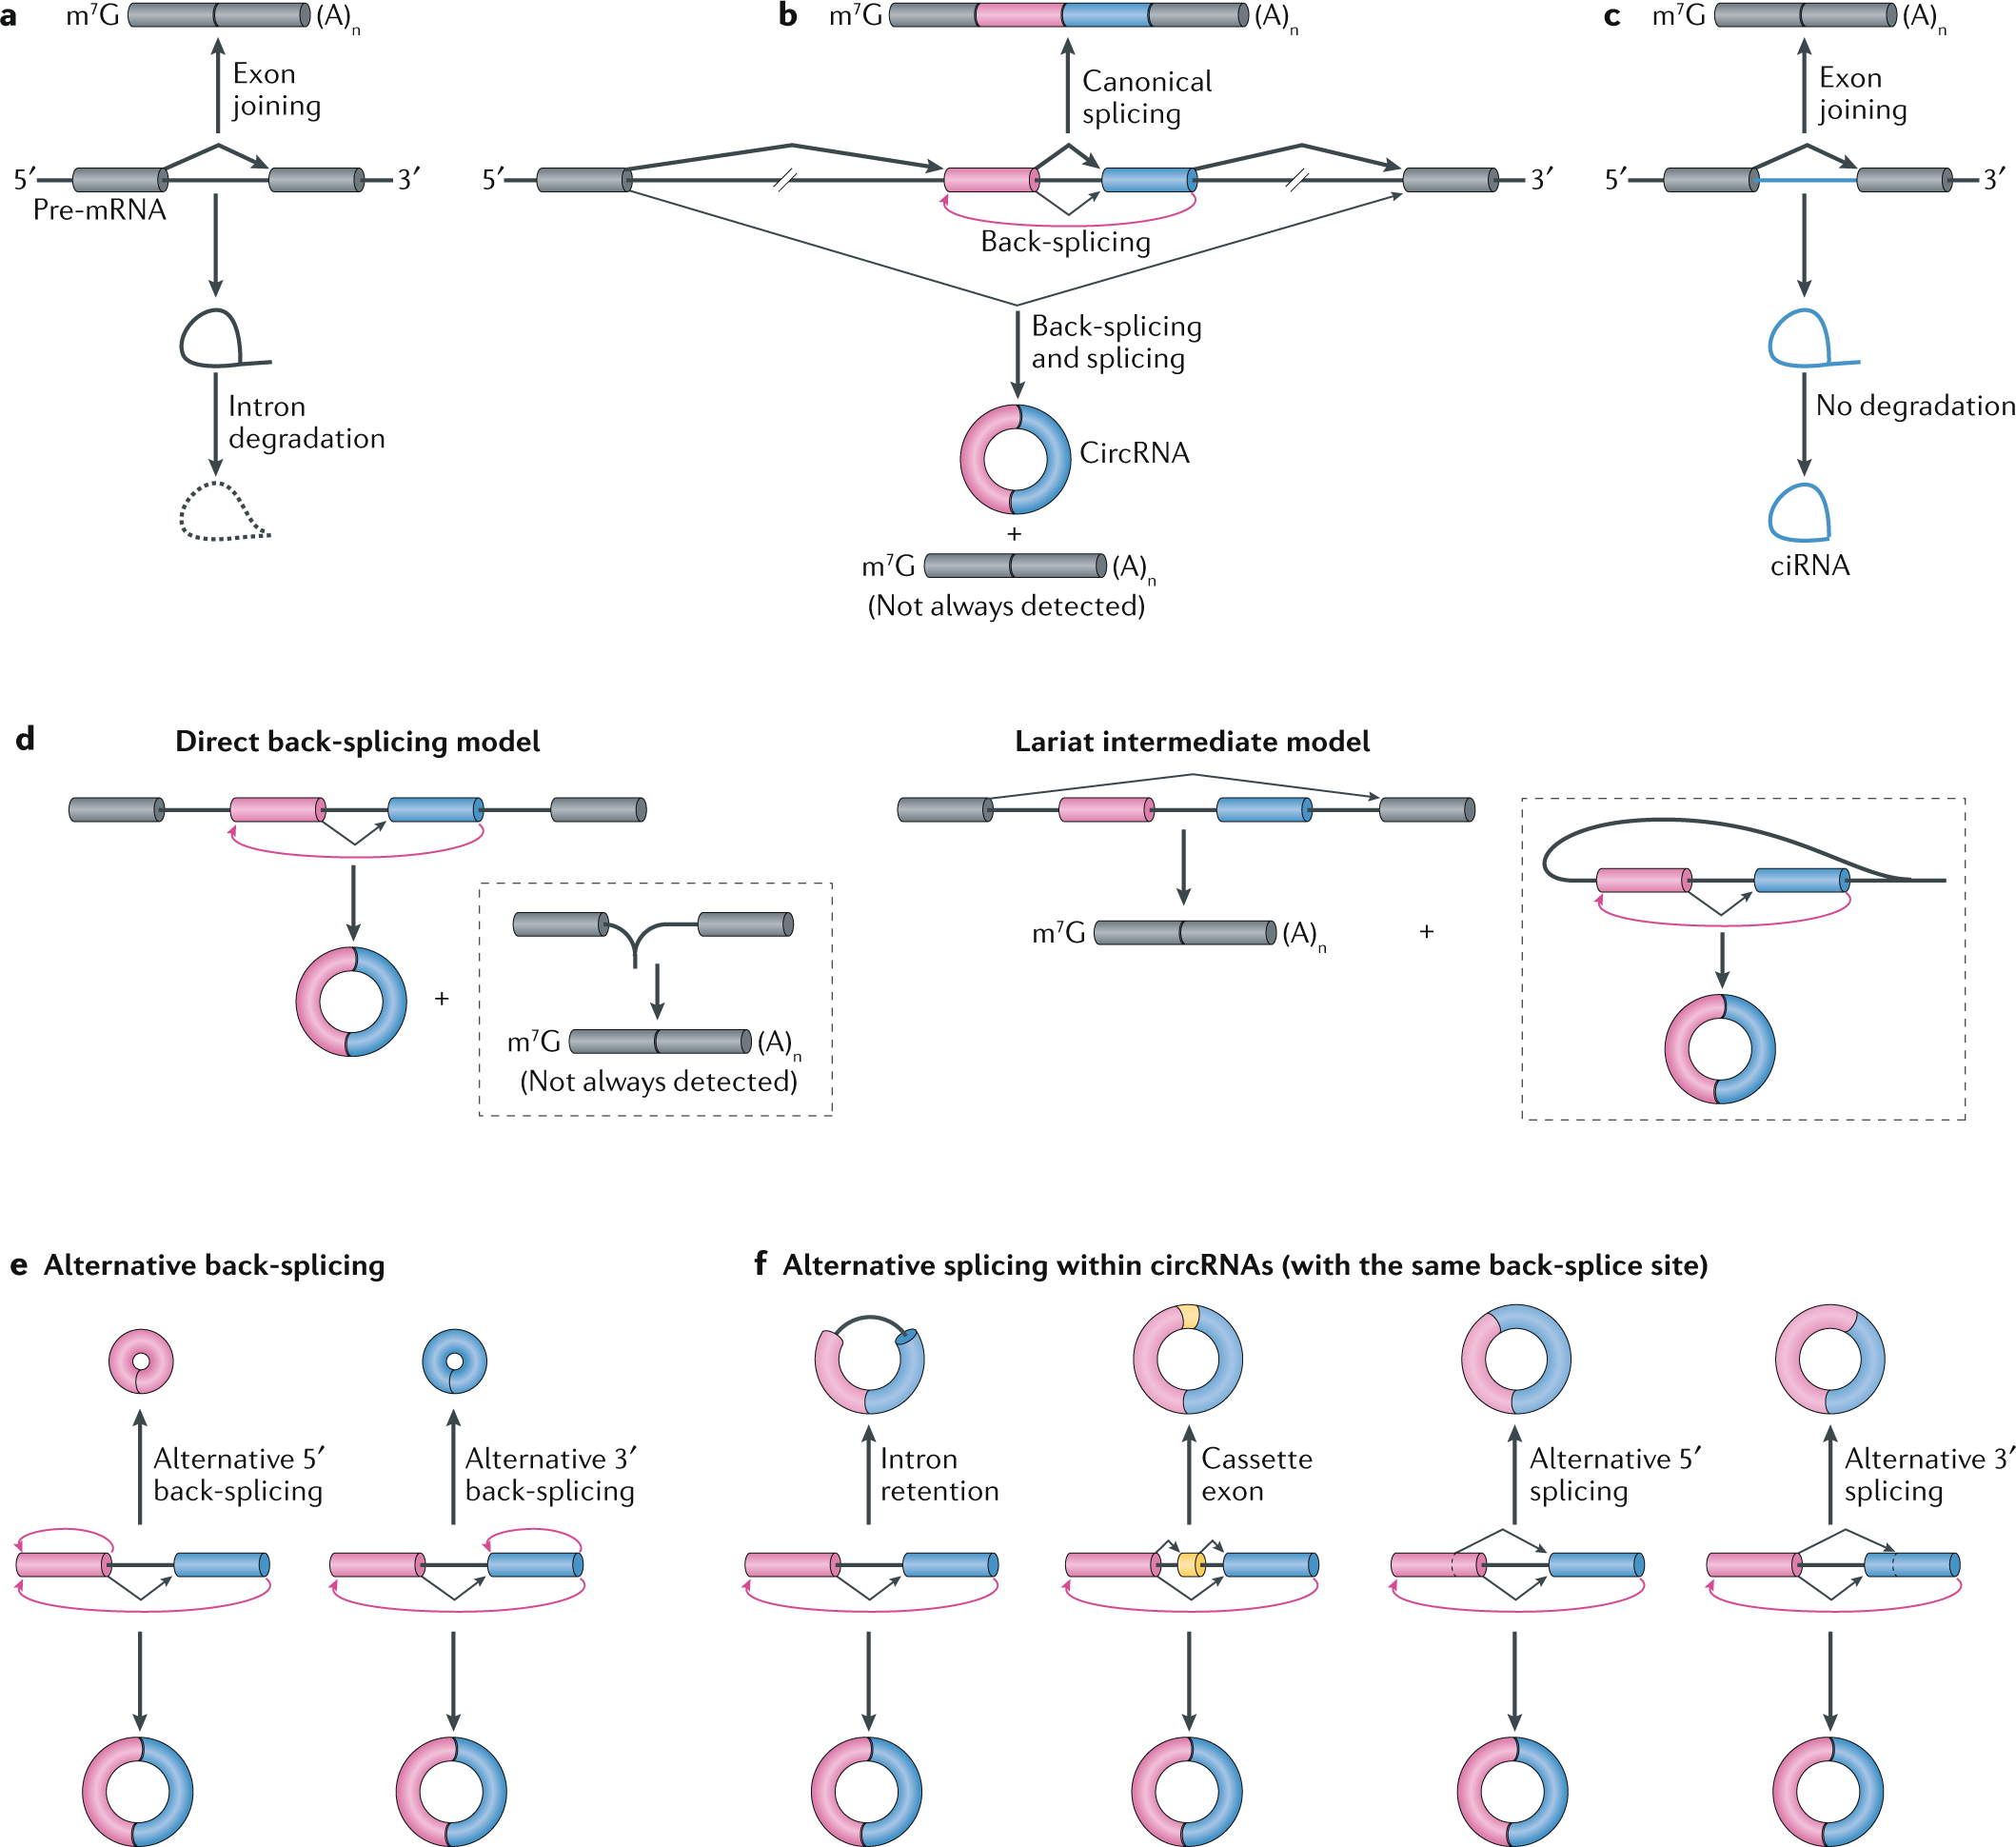
\includegraphics[width=\textwidth]{chapters/background/figures/circRNA-splicing.png}
    \caption{Splicing of circRNAs} % TODO: Add detailed caption
    \label{fig:circRNA_splicing}
\end{figure}

\subsection{Functions}
This subsection describes what functions circRNAs have.

\subsubsection{miRNA sponging}
This subsubsection describes how circRNAs can act as miRNA sponges.

\subsubsection{Protein binding}
This subsubsection describes how circRNAs can bind to proteins.

\subsubsection{Protein coding}
This subsubsection describes how circRNAs can code for proteins.

\subsection{Existing research}
This subsection describes the current state of research on circRNAs.

\section{totalRNA sequencing}
This subsection describes the sequencing method used to identify circRNAs.

\lipsum[2]

\section{Breast cancer}
This section describes what breast cancer is, how it is diagnosed, and what the current treatment options are.
It also gives insights into the current state of research.

\lipsum[3]

\section{Estrogen signaling}
This section describes what estrogen is, how it affects breast cancer, and what the current treatment options are.
It also gives insights into the current state of research.

\lipsum[4]

\section{Related work}
This section describes related work on circRNAs, breast cancer, and estrogen signaling.

\subsection{circRNA-sponging pipeline}
This subsection describes a pipeline for identifying circRNA sponges.